\documentclass[tikz,dvisvgm]{standalone}
\usetikzlibrary{decorations.markings}
\usetikzlibrary{decorations.text}
\usetikzlibrary{shapes,arrows}

\tikzstyle{block} = [draw, fill=white, rectangle, minimum height=3em, minimum width=6em]
\tikzstyle{sum} = [draw, fill=white, circle, node distance=2cm]

\begin{document}
	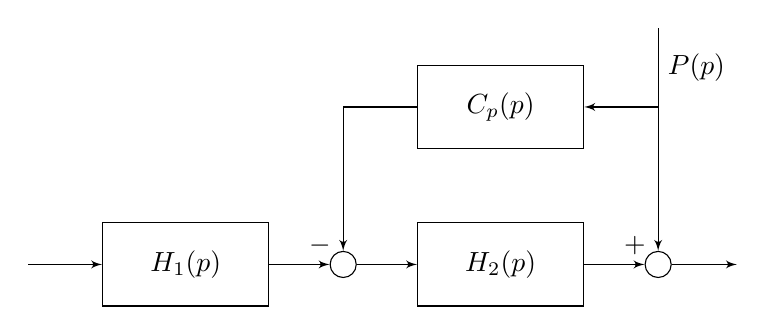
\begin{tikzpicture}[node distance=2cm, >=latex']
		\node[coordinate] (input) at (0,0) {};
		\node[block, right of=input] (H1) {$H_1(p)$};
		\node[sum, right of=H1] (sub1) {};
		\node[block, right of=sub1] (H2) {$H_2(p)$};
		\node[sum, right of=H2] (sum1) {};
		\node[coordinate, right of=sum1, node distance=1cm] (output) {};
		
		\node[coordinate, above of=sum1] (pertub) {};
		\node[coordinate, above of=pertub, node distance=1cm] (pertubin) {};
		\node[block, above of=H2] (C) {$C_p(p)$};
		
		\draw[->] (input) -- (H1);
		\draw[->] (H1) -- node [above right] {$-$} (sub1);
		\draw[->] (sub1) -- (H2);
		\draw[->] (H2) -- node [above right] {$+$} (sum1);
		\draw[->] (sum1) -- (output);
		
		\draw[-] (pertubin) -- node [right] {$P(p)$} (pertub);
		\draw[->] (pertub) -- (sum1);
		\draw[->] (pertub) -- (C);
		\draw[->] (C) -| (sub1);
		
	\end{tikzpicture}
\end{document}
